\chapter{\label{ch:ch03}ГЛАВА 3}

Пример ссылок:
\begin{enumerate}
\item на главу~\ref{ch:ch01};
\item на раздел~\ref{sec:ch01/sec01} главы~\ref{ch:ch01};
\item на раздел~\ref{sec:ch02/sec01} главы~\ref{ch:ch02};
\item на приложение на странице~\pageref{appendix1};
\item на код на странице~\pageref{code:pi-example}.
\end{enumerate}

\section{\label{sec:ch03/sec01}Раздел 1}

\subsection{\label{subsec:ch03/sec01/sub01}Подраздел 1}

\subsection{\label{subsec:ch03/sec01/sub02}Подраздел 2}

\section{\label{sec:ch03/sec02}Раздел 2}

\subsection{\label{subsec:ch03/sec02/sub01}Подраздел 1}

\subsection{\label{subsec:ch03/sec02/sub02}Подраздел 2}

Пример ссылки на рисунок в документе~\ref{fig:example05}.
\begin{figure}[h]
    \centering
    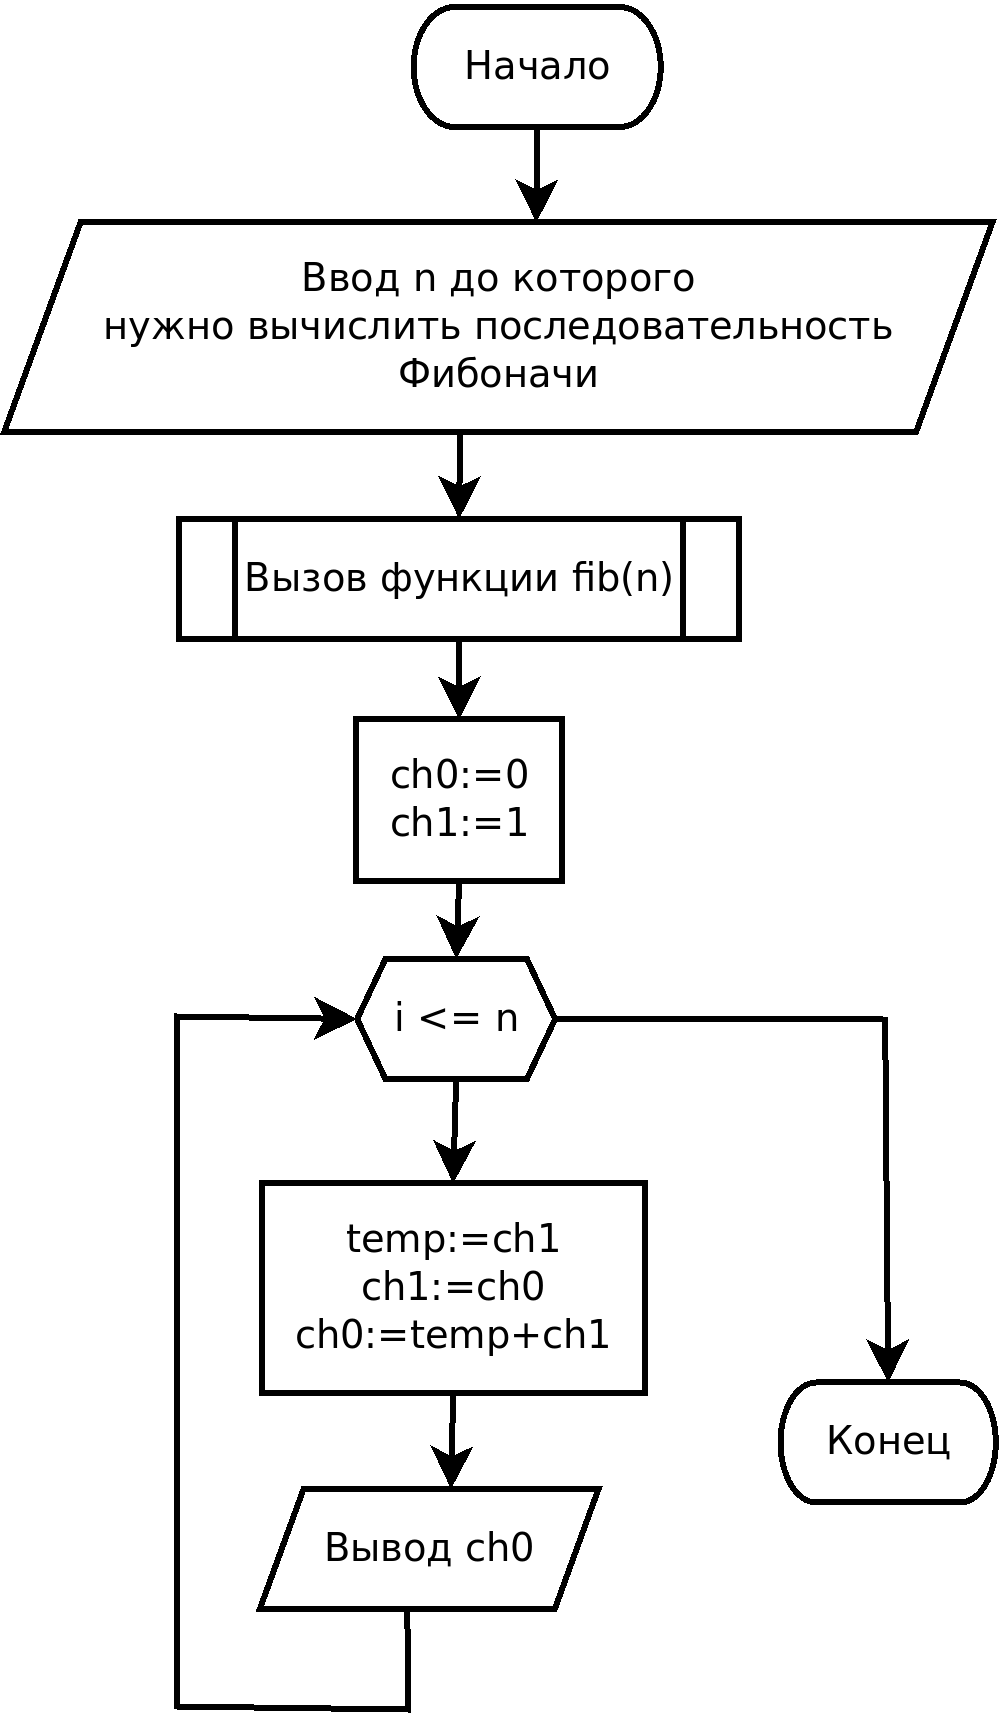
\includegraphics[width=0.5\textwidth]{./images/fibonacci.png}
    \caption{\centering\label{fig:example05}Пример рисунка в формате PNG.}
\end{figure}

Пример ссылки на таблицу в документе~\ref{tab:example05}.
\begin{table}[H]
\caption{\centering\label{tab:example05}Системные требования}
\begin{tabular}{|p{3 cm}|p{3 cm}|p{3 cm}|p{5 cm}|}
\hline
Минимальные требования & 1 & 2 & 3 \\ \hline
Версия операционной системы & 1 & 2 & 3 \\ \hline
Процессор & 1 & 2 & 3 \\ \hline
Графический API & 1 & 2 & 3 \\ \hline
\end{tabular}
\end{table}

Пример ссылки на таблицу в документе~\ref{tab:example06}.
\begin{table}[H]
\caption{\centering\label{tab:example06}Системные требования}
\begin{tabular}{|p{3 cm}|p{3 cm}|p{3 cm}|p{5 cm}|}
\hline
Минимальные требования & 1 & 2 & 3 \\ \hline
Версия операционной системы & 1 & 2 & 3 \\ \hline
Процессор & 1 & 2 & 3 \\ \hline
Графический API & 1 & 2 & 3 \\ \hline
\end{tabular}
\end{table}

Пример использования minted для оформления кода и ссылка на этот код~\ref{code:example05}.
\begin{code}
\captionof{listing}{\centering\label{code:example05}Вычисление последовательности Фибоначчи}
\vspace{-\baselineskip}\begin{minted}{C}
#include <stdio.h>
#include <omp.h>
#define N 100

int main(int argc, char *argv[]) {
  double a[N], b[N], c[N];
  int i;
  omp_set_dynamic(0); // запретить библиотеке openmp менять число потоков во время исполнения
  omp_set_num_threads(10); // установить число потоков в 10
  // инициализируем массивы
  for (i = 0; i < N; i++) {
      a[i] = i * 1.0;
      b[i] = i * 2.0;
  }
  // вычисляем сумму массивов
#pragma omp parallel for shared(a, b, c) private(i)
   for (i = 0; i < N; i++)
     c[i] = a[i] + b[i];

  printf ("%f\n", c[10]);
  return 0;
}
\end{minted}
\end{code}

Пример использования minted для оформления кода и ссылка на этот код~\ref{code:example06}.
\begin{code}
\captionof{listing}{\centering\label{code:example06}Сложение двух массивов параллельно десятью потоками (пример из https://ru.wikipedia.org/wiki/OpenMP)}
\vspace{-\baselineskip}\begin{minted}{C}
#include <stdio.h>
#include <omp.h>
#define N 100

int main(int argc, char *argv[]) {
  double a[N], b[N], c[N];
  int i;
  omp_set_dynamic(0); // запретить библиотеке openmp менять число потоков во время исполнения
  omp_set_num_threads(10); // установить число потоков в 10
  // инициализируем массивы
  for (i = 0; i < N; i++) {
      a[i] = i * 1.0;
      b[i] = i * 2.0;
  }
  // вычисляем сумму массивов
#pragma omp parallel for shared(a, b, c) private(i)
   for (i = 0; i < N; i++)
     c[i] = a[i] + b[i];

  printf ("%f\n", c[10]);
  return 0;
}
\end{minted}
\end{code}
